\begin{abstract}
Integrated scheduling of processing and transport in flexible job shops almost always treats travel times as a location-indexed constant matrix.
Once a finite fleet shares a sparse corridor network, travel time is the outcome of conflict-free path planning---routing, in this paper---because one job's occupancy delays others.
This paper studies a class in which each operation may use one of several robotic arms that are homogeneous in capability and heterogeneous in efficiency, while AGVs must travel conflict-free.
Machine flexibility then becomes an operational trade-off: when the corridor to a fast arm is congested, a slower arm with better connectivity may be the better assignment.

A \emph{closed-loop bilevel framework} connects the two decisions along an evaluation path and a decision path.
The upper level assigns machines and sequences operations; the lower level generates conflict-free paths by time-window reservation.
\emph{Routing-in-the-loop evaluation} takes the fitness of each candidate as the makespan after that routing, so yielding wait enters the search objective.
\emph{Reservation-table-aware dispatching} selects a vehicle by trial-querying both transport legs on the reservation table, not by unimpeded travel time.
Two low-overhead optimizations---admissible lower-bound pruning and winner-path reuse---change neither the selected vehicle nor the timetable.

On \NCases{} controlled instances of one size, with contention from \ContentionLo{} to \ContentionHi{}, a four-level ladder, \NSeeds{} seeds, and an equal wall-clock budget, the closed loop reduces makespan by \GainLoopRule{} ($p\PLoopRule$) relative to the open loop;
within the closed loop, reservation-table-aware dispatching reduces it by a further \GainProbeLoop{} ($p\PProbeLoop$);
end-to-end the reduction is \GainEndToEnd{} (\WinEndToEnd{} wins, \LoseEndToEnd{} losses, $p\PEndToEnd$), close to the independent product \GainIndepProduct{}.
The closed loop is the main effect and remains significant per instance on \CellsSigLoopAdj{} instances after correction; dispatching is a much smaller secondary effect, significant only when all instances are pooled and on none individually.
The two are near-additive; no positive interaction is detected.
\end{abstract}

%%
%% The code below is generated by the tool at http://dl.acm.org/ccs.cfm.
%% Please copy and paste the code instead of the example below.
%%
%% Previous CCS block described a different paper; left commented.
%% concept_id must come from dl.acm.org/ccs.cfm, not be typed.  If submitting
%% to ACM, regenerate; suggested concepts:
%%   Theory of computation~Scheduling algorithms            (significance 500)
%%   Applied computing~Industry and manufacturing           (significance 300)
%%   Computing methodologies~Planning and scheduling        (significance 300)
%% Drop the block for a non-ACM venue.
%
% \begin{CCSXML}
% <ccs2012>...</ccs2012>
% \end{CCSXML}
% \ccsdesc[500]{Theory of computation~Scheduling algorithms}

%%
%% Keywords. The author(s) should pick words that accurately describe
%% the work being presented. Separate the keywords with commas.
\keywords{flexible job shop scheduling, conflict-free routing, closed-loop bilevel framework, routing-in-the-loop evaluation, reservation-table-aware vehicle dispatching}

%% ===================== Authors =====================
%% acmart errors with "No author given" and empties the running head if this
%% block is missing.  Confirm names and order before submission.  For double
%% blind, use \documentclass[...,anonymous]{acmart}; do not delete the block.
\author{Qi Yu}
%%\authornote{.}
%%\authornotemark[1]
\email{230240012@seu.edu.cn}
\orcid{0009-0008-7843-6345}
%%\authornote{corresponding author}
\affiliation{%
	\institution{School of Cyber Science and Engineering, Southeast University}
	\city{Nanjing}
	\state{Jiangsu}
	\country{PR China}
}
\author{Wei Li}
\orcid{0009-0001-0949-329X}
\email{xchlw@seu.edu.cn}
\authornote{corresponding author}
\affiliation{%
	\institution{School of Computer Science and Engineering, Southeast University}
	\city{Nanjing}
	\state{Jiangsu}
	\country{PR China}
}

%% Running-head short authors.  Unset, acmart falls back to "Trovato et al."
\renewcommand{\shortauthors}{Qi et al.}



%\Acknowledgements{This work was supported partly by Key Laboratory of Computer Network and Information Integration (Southeast University) of Ministry of Education of China under Grants NO. 93K-9 and Jiangsu Provincial Key Laboratory of Network and Information Security under Grants No.BM2003201.}


%% Venue fills the three received dates.  Do not keep the old 2025 dates.
\received{XX XX 2026}
\received[revised]{XX XX 2026}
\received[accepted]{XX XX 2026}

%%
%% This command processes the author and affiliation and title
%% information and builds the first part of the formatted document.
\maketitle
\section{Introduction}
\label{sec:Chapter_I}

\subsection{Motivation and gap}

Flexible job shop scheduling with transportation has long treated travel time as a constant, read from a matrix indexed by location pairs---the dominant convention~\cite{xin2025review}, still widely used~\cite{meng2025cp,qin2026knowledge,fu2025integrated}.
The assumption is reasonable when vehicles rarely meet.
Real shops are not built that way: a few vehicles share a sparse corridor network, and a single-lane segment cannot be used in both directions at once; once fleet density is high enough, the fleet's own traffic becomes the main delay~\cite{kim2026congestion}.
Travel time is then the outcome of two decisions---which path a vehicle takes (conflict-free path planning; routing, in this paper) and who first reserved the contended segment---not the distance between two points.

That coupling can be optimized only if the scheduler can change the assignment.
When an operation may use any arm in an option set, and the processing time depends on the arm, the assignment selects both the destination and the duration.
Under a constant matrix the comparison is arithmetic (shorter processing plus longer travel, or the reverse).
With corridor contention the wait on the path to a fast arm is invisible to the matrix, so a slower arm with better connectivity may be better---and the ranking may flip again at a different congestion level.
The trade-off needs both ingredients: heterogeneous optional arms, and distinct paths on which vehicles contend.

Figure~\ref{fig:motivating} reports two readings on a recomputable instance ($4$ jobs, $2$ AGVs).
The first is the unimpeded chain of J1 alone (panel~(a)): $\mathrm{LU}\to v_1\to v_2\to\mathrm{M1}$ is $2(1+\tau+1)+3=19$; $\mathrm{LU}\to v_1\to\mathrm{M2}$ is $2(1+2)+14=20$.
The fast arm wins that comparison iff $19<20$, so $\tau=6$ and $t^P_{\text{fast}}=3$ already force $t^P_{\text{slow}}\ge 14$.
The second is instance $C_{\max}$ (panel~(b)): last return to LU, same decoder, not $19$ or $20$ and not a sum of processing times.
On the constant matrix the two AGVs stay in step if J1 goes to M1 (last return $41$) and one AGV is held at M2 if J1 goes there (last return $54$).
Conflict-free routing on the same pair occupies the exclusive trunk when J1 uses M1 (last return $95$) and avoids it when J1 uses M2 (last return $60$).
Neither assignment nor sequence has changed; only the evaluation has.

\begin{figure*}[t]
\centering
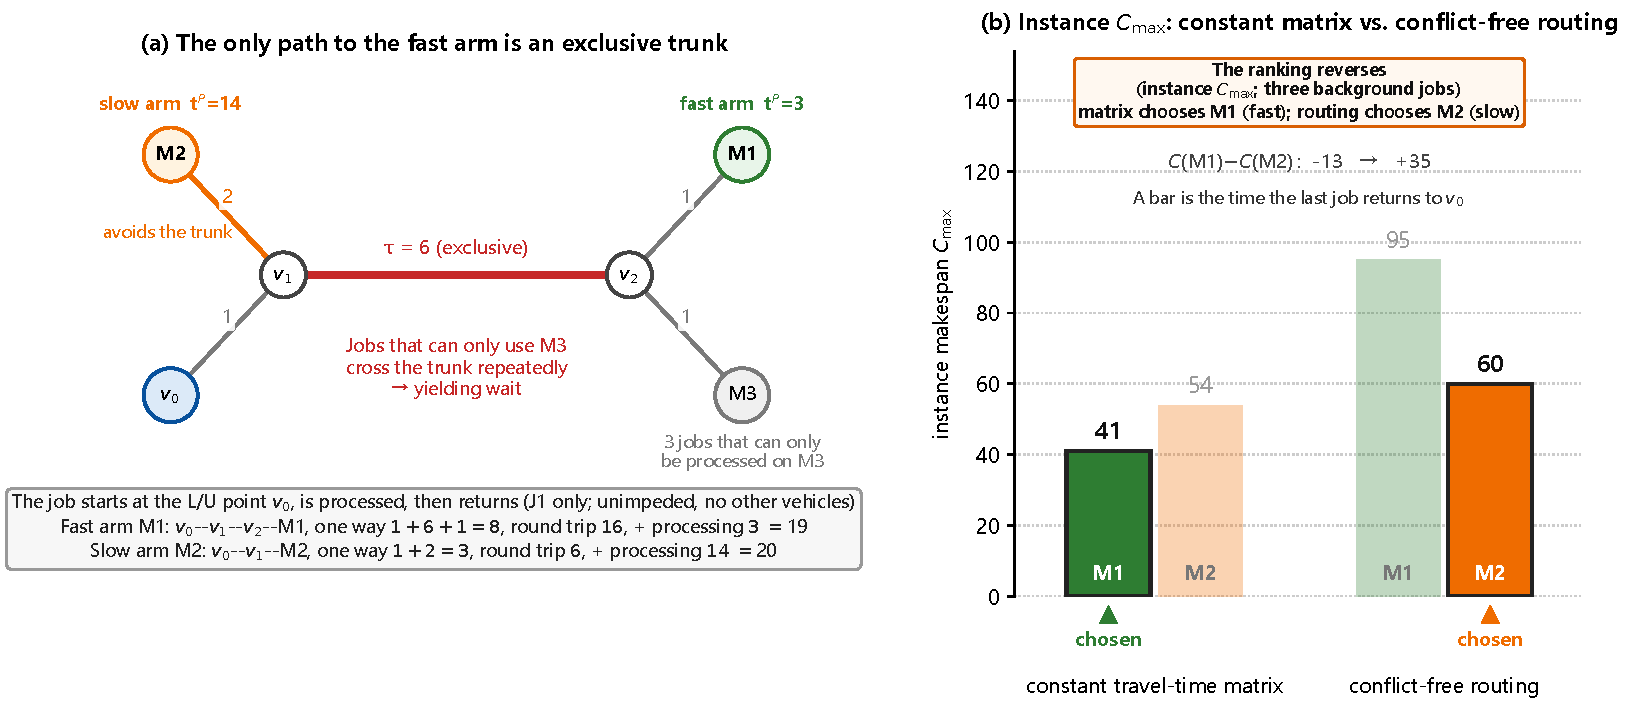
\includegraphics[width=\textwidth]{fig/fig_motivating.pdf}
\Description{Two panels. The left panel is a shop network and J1's unimpeded chain ($19$ vs $20$). The right panel is instance makespan (last return to LU) for the same two assignments: $41$ vs $54$ on the constant matrix, $95$ vs $60$ under conflict-free routing.}
\caption{Motivating instance: two readings of the same pair of assignments.
(a)~J1's unimpeded chain: exclusive trunk to M1 ($2(1+6+1)+3=19$) versus the short corridor to M2 ($2(1+2)+14=20$); the bottom box is this comparison, not the bars in~(b).
(b)~Instance $C_{\max}$ (last return to LU): the constant matrix ranks M1 better ($41$ vs $54$); conflict-free routing ranks M2 better ($95$ vs $60$).
An \emph{existence demonstration}: of $1200$ nearby parameter combinations, $205$ ($17\%$) reverse.}
\label{fig:motivating}
%% From fig/fig_motivating.py and clbs/output/motivating.json
%% (clbs/tools/motivating.py --sweep; same decoder as the paper).
%% Panel (b) numbers are not schematic: unimpeded matrix =
%% decode(conflict_free=False), conflict-free routing = decode(conflict_free=True).
%% Instance: 4 jobs / 3 arms / 6 nodes / 5 corridors / 2 AGVs, delta_return=1,
%% rule-based dispatching.  Do not reuse fig/fig_intro_problem_new.pdf
%% (previous paper, proximity-vs-availability, not corridor contention).
\end{figure*}

Existing work typically treats flexible-job-shop scheduling or conflict-free travel, not both; when they are combined, the assignment is usually fixed first and routing then absorbs the contention, so delay cannot revise the schedule.
An exact method already formulates both in one problem and solves small instances to proven optimality~\cite{vanos2026exact}; this paper adopts that problem setting, and its contribution is the solver, not the problem definition.
Beyond that exact size, heuristics still schedule then resolve~\cite{sun2023integrated}, or write realized durations back onto the time axis of the current solution only, on a benchmark with one machine per operation~\cite{li2026framework}.
The trade-off in which flexibility, heterogeneous efficiency, and corridor contention are present at once, and every candidate is ranked by the makespan after yielding wait, is therefore still open at heuristic size.
The literature position is in Section~\ref{sec:Chapter_II}.

\subsection{Approach and contributions}

This paper connects the two levels along an evaluation path and a decision path, and measures each under an equal wall-clock budget.
The upper level assigns machines and sequences operations; the lower level generates conflict-free paths by time-window reservation.

The \emph{evaluation path} takes the fitness of each candidate as the makespan after conflict-free routing, so yielding wait enters the search objective.
One such decode is more than an order of magnitude more expensive than a lookup of the unimpeded matrix; under a fixed compute budget, a higher cost per evaluation leaves fewer evaluations.
\cite{li2026framework} lists a fully iterative loop as future work, but does not report that cost or its effect on makespan.

The \emph{decision path} uses \emph{reservation-table-aware dispatching}: both transport legs (empty pickup, then loaded delivery) are trial-queried on the reservation table without writing the timetable, and the vehicle with the earliest feasible delivery is selected, replacing the idle-first rule of~\cite{li2026framework}.
Two output-preserving optimizations---admissible lower-bound pruning and winner-path reuse---keep each evaluation low-overhead.
A surcharge on occupied corridor--time slots, and reassignment or staggering from the yield record, were also implemented; neither further reduces makespan under the same budget (Section~\ref{sec:Chapter_V}).

Four configurations in a $2\times 2$ design (open or closed loop $\times$ rule-based or reservation-table-aware dispatching) separate the two paths.
\textbf{B0} is open-loop planning plus actual execution~\cite{li2026framework};
\textbf{B0+} replaces only vehicle assignment on a frozen schedule~\cite{sun2023integrated};
\textbf{B1} is closed-loop planning plus rule-based dispatching;
\textbf{B2} is the method of this paper.
Every schedule is executed by the same conflict-free planner; what is compared is the realized makespan.
Moving congestion into the search reduces makespan by \GainLoopRule{} ($p\PLoopRule$), the larger effect;
within the closed loop, reservation-table-aware dispatching reduces it by a further \GainProbeLoop{} ($p\PProbeLoop$), a smaller but still significant effect;
end-to-end the reduction is \GainEndToEnd{} (\WinEndToEnd{} wins, \LoseEndToEnd{} losses, $p\PEndToEnd$).
The two speed-ups give a factor of \SpeedupProbe{}, cut router calls by \RouteCallCut{}, and lower the cost multiple from \CostMultBefore{} to \CostMultAfter{}.
The two factors are near-additive (\GainEndToEnd{} close to \GainIndepProduct{}) and are not substitutes: open-loop dispatching gives only \GainProbeOpen{} ($p\PProbeOpen$).
After Holm correction by family, the closed loop remains significant on \CellsSigLoopAdj{}/\NCases{} instances; dispatching is significant only when instances are pooled and on none individually (\CellsSigProbe{} before correction).
With \NSeeds{} seeds per instance, the sample cannot yet determine on which class of instances the dispatching gain is stable.
The protocol is in Section~\ref{sec:protocol}; per-instance results are in Section~\ref{sec:whichcongestion}.

The four contributions, restated with supporting numbers in Section~\ref{sec:contributions}, are:
\textbf{(1)~Instances:}~a controllable characterization of the reassignment trade-off---how high contention must be before counting yielding wait in the schedule yields a gain;
\textbf{(2)~Evaluation:}~routing-in-the-loop evaluation, so every candidate is ranked by the makespan after conflict-free routing;
\textbf{(3)~Dispatching:}~reservation-table-aware dispatching with two output-preserving speed-ups, so the trial query remains affordable under the same wall-clock budget;
\textbf{(4)~Evidence:}~the two paths differ in magnitude, are near-additive, and are not substitutes---the closed loop is larger and robust per instance, while dispatching is significant only when pooled.

The notation of the paper is collected in Table~\ref{tab:notation}.



\section{Related work}
\label{sec:Chapter_II}

Two strands sit next to this paper: flexible job shop scheduling with transportation times, and conflict-free routing of exogenous tasks.
Work that writes both into one problem is scarce; Table~\ref{tab:related} places the present solver against that literature.

\subsection{Two strands}

FJSP\_PT extends FJSP by bringing material movement into the schedule~\cite{xin2025review,dauzereperes2024fjsp}.
Public benchmarks are collected by Homayouni and Fontes~\cite{homayouni2021production}.
The dominant convention is a constant travel-time matrix: a vehicle needs a fixed $t(a,b)$, independent of corridor occupancy, so vehicles enter only as capacity resources.
Meng et al.~\cite{meng2025cp} close 29 previously open benchmarks and improve 27 best-known solutions; Qin et al.~\cite{qin2026knowledge} guide a local search by AGVs and a critical path still computed on matrix times; Fu et al.~\cite{fu2025integrated} decide production and logistics jointly, without making transport duration depend on the schedule.
These assumptions ``reduce the complexity of the problem and even change its nature''~\cite{xin2025review}: when the fleet is large enough, arrival times are affected by congestion, and a plan that ignores that dependence need not be feasible on the actual corridors.
This strand has machine flexibility, but no yielding wait.
% [ref_check: key=xin2025review; claim="review covers progress through 2023; constant matrix is dominant; the matrix reduces complexity and can change the nature of the problem"; need=quote]
% [ref_check: key=meng2025cp; claim="closes 29 previously open benchmarks and improves 27 best-known solutions"; need=quote]

The other strand takes corridor contention as the object.
Optimal multi-agent path finding is NP-hard~\cite{gao2023mapf}; Safe Interval Path Planning extends single-vehicle routing to continuous-time road networks~\cite{kasaura2022sipp}.
Zhang et al.~\cite{zhang2024guidance} steer lifelong agents with offline-learned edge weights; Kim and Kim~\cite{kim2026congestion} give density-based congestion-aware dispatching.
Surveys list dispatching as independent of path planning~\cite{lu2022agv} and task allocation as adjacent to it~\cite{fragapane2021planning}.
Release times and endpoints are inputs: the router cannot change the assignment that produced the tasks.
Congestion is usually a proxy---local density~\cite{kim2026congestion} or offline edge weights~\cite{zhang2024guidance}---not the yield that names a corridor, an interval, and the transport that occupied it first.
This strand has genuine conflict-free routing, but no flexibility.
% [ref_check: key=zhang2024guidance,kim2026congestion; claim="release times and endpoints are exogenous; congestion is density or offline edge weights"; need=quote]

\subsection{Integration and our position}

van Os and Basten~\cite{vanos2026exact} formalize FJSP with conflict-free transportation: optional machines, location-dependent processing times, and conflict-free travel.
A logic-based Benders solver (constraint-programming master, integer-programming routing subproblem, conflict-driven cuts) solves most benchmarks to proven optimality and improves about half of them by at least $10\%$ over prior heuristics, within the size the exact decomposition can reach.
This paper adopts that setting; the contribution is a heuristic that, beyond that size, sends routing delay back into every scheduling candidate.
% [ref_check: key=vanos2026exact; claim="most benchmarks solved to proven optimality; about half improve makespan by at least 10% over prior heuristics"; need=quote]

Sun et al.~\cite{sun2023integrated} still fix assignment and sequence first, then resolve conflicts with a genetic AGV encoding and time-window Dijkstra; the second stage cannot revise the first.
Li et al.~\cite{li2026framework} write realized durations back onto the current solution only, on a one-machine-per-operation benchmark.
The remaining gap is how the routing result enters the schedule: whether every candidate is evaluated by actual routing, and whether the assignment can change from that evaluation.
% [ref_check: key=sun2023integrated; claim="second-stage conflict resolution does not revise first-stage schedule or assignment"; need=quote]
% [ref_check: key=li2026framework; claim="feedback is time only; the experimental benchmark has one optional machine per operation"; need=quote]

Critical-chain local search is mature~\cite{otala2021graph,tamssaouet2023neighborhood,qin2026knowledge}, but a chain on a constant matrix cannot name a corridor; after time-window reservation it can.
On instance design, \cite{xin2025review} notes that published instances ``differ mainly in size'' and lists $\bar{T}_t/\bar{T}_p$ as likely to affect performance; this paper also varies how much of the congestion is assignment-related (Section~\ref{sec:Chapter_V}).
% [ref_check: key=xin2025review; claim="instances differ mainly in size; T_t/T_p is listed as likely to affect performance"; need=quote]

\begin{table}[t]
  \caption{Related work versus this paper.
Machine heterogeneity: optional machines with machine-dependent processing times.
Coupling frequency: how often, and in which direction, the routing result enters the schedule.}
\label{tab:related}
%% Hand-maintained table: no generator.  Any row change must match Section 2.2.
\footnotesize
\begin{tabular}{@{}lclll l@{}}
\toprule
Work class & Ref. & Machine het. & Vehicle contention & Coupling freq. & Feedback content \\
\midrule
FJSP\_PT metaheuristics & \cite{meng2025cp,qin2026knowledge,fu2025integrated}
  & yes & constant matrix & --- & --- \\
Lifelong MAPF & \cite{gao2023mapf,zhang2024guidance}
  & --- & conflict-free & tasks exogenous & edge weights \\
Congestion-aware dispatching & \cite{kim2026congestion}
  & no & density proxy & one-way & congestion penalty \\
Two-stage FJSP + routing & \cite{sun2023integrated}
  & yes & conflict-free & one-way & none \\
RL scheduling + PBS & \cite{li2026framework}
  & no & conflict-free & one-shot correction & arrival times \\
Exact LBBD & \cite{vanos2026exact}
  & yes & conflict-free & master--subproblem & conflict-driven cuts \\
\textbf{This paper} &
  & yes & conflict-free & every candidate & realized time + trial query \\
\bottomrule
\end{tabular}
\end{table}


